\chapter{Nahfeld}\label{ch:nahfeld}
\index{Nahfeld}%

Neben den Effizienzen berechnet \FG{} die Felder $\mathbf E$ und $\mathbf H$ in der Struktur und in ihrer Umgebung.
Das zeigt Feldüberhöhungen, Resonanzen, Moden und Absorptionsorte.

\section{Schnitte}
\begin{center}
\begin{tikzpicture}[scale=1.4]
  % 3D-artige Zelle
  \draw[fill=gray!20] (0,0) -- (3,0) -- (3.8,0.6) -- (0.8,0.6) -- cycle;
  \draw[fill=blue!25] (0,0) -- (3,0) -- (3,1.2) -- (0,1.2) -- cycle;
  \draw[fill=blue!15] (3,0) -- (3.8,0.6) -- (3.8,1.8) -- (3,1.2) -- cycle;
  \draw[fill=blue!8] (0,1.2) -- (3,1.2) -- (3.8,1.8) -- (0.8,1.8) -- cycle;
  % vertikaler Schnitt
  \draw[very thick,red!70!black,fill=red!15,opacity=0.7] (0.4,-0.6) -- (3.4,-0.6) -- (3.4,2.4) -- (0.4,2.4) -- cycle;
  \node[red!70!black,anchor=west] at (3.5,2.2) {\small vertikaler Schnitt: $z=z_0$, Karte $(x,y)$};
  % horizontaler Schnitt
  \draw[very thick,fgblue,fill=fgblue!15,opacity=0.7] (-0.3,0.7) -- (3.0,0.7) -- (4.1,1.5) -- (0.8,1.5) -- cycle;
  \node[fgblue,anchor=west] at (4.2,1.1) {\small horizontaler Schnitt: $y=y_0$};
  \node[fgblue,anchor=west] at (4.2,0.75) {\small 1D: Linie $u(x)$; 2D: Karte $(x,z)$};
  \draw[->] (-0.8,-0.4) -- (-0.3,-0.4) node[right] {\scriptsize$x$};
  \draw[->] (-0.8,-0.4) -- (-0.8,0.1) node[above] {\scriptsize$y$};
  \draw[->] (-0.8,-0.4) -- (-0.5,-0.2) node[above right] {\scriptsize$z$};
\end{tikzpicture}
\end{center}
Je Rechnung gibt es zwei Schnitte:
\begin{itemize}
  \item den \textbf{vertikalen Schnitt} bei $z=z_0$: eine Karte über $x$ und $y$ (bei 1D-Gittern spielt $z_0$ keine Rolle),
  \item den \textbf{horizontalen Schnitt} bei $y=y_0$: bei 1D-Gittern eine Linie über $x$, bei 2D-Gittern eine Karte über
        $x$ und $z$.
\end{itemize}

\section{Konfiguration}
\begin{lstlisting}[language=json]
"nearfield": {
  "enabled": true,
  "horizontal_y_um": 0.125,      // Lage y0 des horizontalen Schnitts
  "vertical_z_um": 0.0,          // Lage z0 des vertikalen Schnitts
  "y_range_um": [-0.3, 0.6],     // y-Bereich des vertikalen Schnitts
  "nx": 400, "ny": 360, "nz": 200,
  "periods": 2,                  // Zahl der dargestellten Perioden
  "reconstruction": "fff",       // "fff" oder "direct"
  "field": "total"               // "total" oder "scattered" (isolierte Strukturen)
}
\end{lstlisting}
\begin{center}
\small
\begin{tabularx}{\linewidth}{lllY}
\toprule
Schlüssel & Typ & Standard & Bedeutung \\
\midrule
\key{enabled} & bool & \val{false} & Nahfeld berechnen \\
\key{horizontal\_y\_um} & Zahl & 0 & $y_0$ (im Substrat negativ) \\
\key{vertical\_z\_um} & Zahl & 0 & $z_0$ (nur 2D wirksam) \\
\key{y\_range\_um} & Liste & $[-0{,}2;\,0{,}5]$ & $y$-Bereich der vertikalen Karte \\
\key{nx}, \key{ny}, \key{nz} & Zahl & 400, 300, 200 & Punkte je Achse (über alle dargestellten Perioden) \\
\key{periods} & Zahl & 1 & Perioden in $x$ (und $z$) \\
\key{reconstruction} & Text & \val{"fff"} & Rekonstruktion der Felder (siehe unten) \\
\key{field} & Text & \val{"total"} & \val{scattered}: nur das Streufeld (Abschnitt~\ref{sec:pml}) \\
\key{quantities} & Liste & & Wunschliste der Größen; geschrieben werden derzeit stets alle \\
\bottomrule
\end{tabularx}
\end{center}
Das Nahfeld wird für den \textbf{ersten Scanpunkt} berechnet (bei Sweeps: des ersten Sweep-Werts). Für mehrere
Wellenlängen rechnen Sie mehrere Konfigurationen oder nutzen Python.

\section{Rekonstruktion: \texttt{fff} oder \texttt{direct}}
\index{Nahfeld!Rekonstruktion}%
An einer Materialgrenze springt die Normalkomponente von $\mathbf E$; stetig ist $\mathbf D_\perp=\varepsilon
\mathbf E_\perp$. Eine abgeschnittene Fourierreihe kann einen Sprung nur mit Gibbs-Schwingungen darstellen.
\begin{description}
  \item[\val{fff}] (Standard) rekonstruiert die stetigen Größen (tangentiales $\mathbf E$, normales $\mathbf D$)
        und berechnet daraus $\mathbf E$. Die Felder sind an Grenzen glatt und physikalisch richtig.
  \item[\val{direct}] summiert die Fourierreihe von $\mathbf E$ direkt. An Wänden entstehen Überschwinger (beim Sprung
        von $D_x$ an Lamellenwänden etwa 300\,\%). Nur für Vergleiche.
\end{description}

\section{Ausgabedateien}\label{sec:nf-dateien}
\cmd{fgsolve} schreibt je Schnitt ein Verzeichnis \file{nearfield\_vertical/} bzw.\ \file{nearfield\_horizontal/} in
\key{output.dir}:
\begin{center}
\small
\begin{tabularx}{\linewidth}{llY}
\toprule
Datei & Typ & Inhalt \\
\midrule
\file{Ex.npy} \ldots{} \file{Ez.npy} & complex128 & elektrisches Feld, bezogen auf $|\mathbf E_{\text{inc}}|=1$ \\
\file{Hx.npy} \ldots{} \file{Hz.npy} & complex128 & magnetisches Feld als $Z_0\mathbf H$ (gleiche Größenordnung wie $\mathbf E$) \\
\file{absE2.npy}, \file{absH2.npy} & float64 & $|\mathbf E|^2$, $|Z_0\mathbf H|^2$ \\
\file{Sy.npy} & float64 & $S_y=\tfrac12\operatorname{Re}(\mathbf E\times\mathbf H^*)_y$ (negativ = abwärts) \\
\file{material.npy} & float64 & $\operatorname{Re}\varepsilon$ in jedem Punkt (zeigt die Geometrie) \\
\file{meta.json} & JSON & Achsen (\texttt{axis1}, \texttt{axis2} mit Werten in \textmu m), Schnitt, $\lambda$, Normierung \\
\bottomrule
\end{tabularx}
\end{center}
Karten haben die Form \texttt{(len(axis2), len(axis1))} in C-Reihenfolge, Linien die Form \texttt{(len(axis1),)}.
Beim vertikalen Schnitt ist \texttt{axis1} $=x$ und \texttt{axis2} $=y$.

\textbf{Mit numpy laden.}
\begin{lstlisting}[style=py]
import json, numpy as np
d = "out/nearfield_lamellar_1d/nearfield_vertical"
meta = json.load(open(f"{d}/meta.json"))
x = np.array(meta["axes"]["axis1"]["values_um"])
y = np.array(meta["axes"]["axis2"]["values_um"])
E2 = np.load(f"{d}/absE2.npy")            # Form (len(y), len(x))
eps = np.load(f"{d}/material.npy")
print("max |E|^2 =", E2.max(), "bei y =", y[np.unravel_index(E2.argmax(), E2.shape)[0]])
\end{lstlisting}

\section{Darstellung mit \texttt{plot\_nearfield.py}}
\begin{lstlisting}[style=shell]
scripts/plot_nearfield.py out/nearfield_lamellar_1d/nearfield_vertical --quantity absE2 --out e2.png
scripts/plot_nearfield.py DIR --quantity Ex --part re|im|abs|phase
\end{lstlisting}
Das Skript zeichnet die Materialgrenzen aus \file{material.npy} als weiße Linien ein.

\begin{figure}[h]
\centering
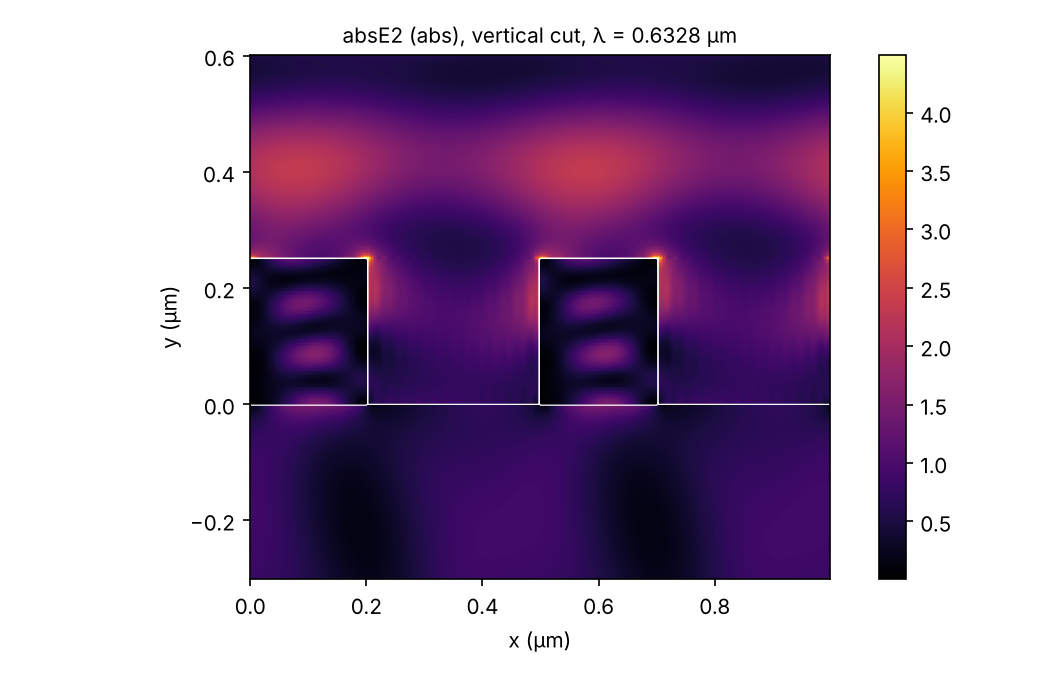
\includegraphics[width=0.68\linewidth]{fig/nf1d_vertical.png}
\caption{$|\mathbf E|^2$ im vertikalen Schnitt durch Siliziumlamellen auf Glas (\file{examples/nearfield\_lamellar\_1d.json},
TM, $\lambda=0{,}6328$\um, zwei Perioden). An den oberen Kanten der Stege ist das Feld stark überhöht; im Silizium
bildet sich eine Stehwelle.}
\end{figure}

\begin{figure}[h]
\centering
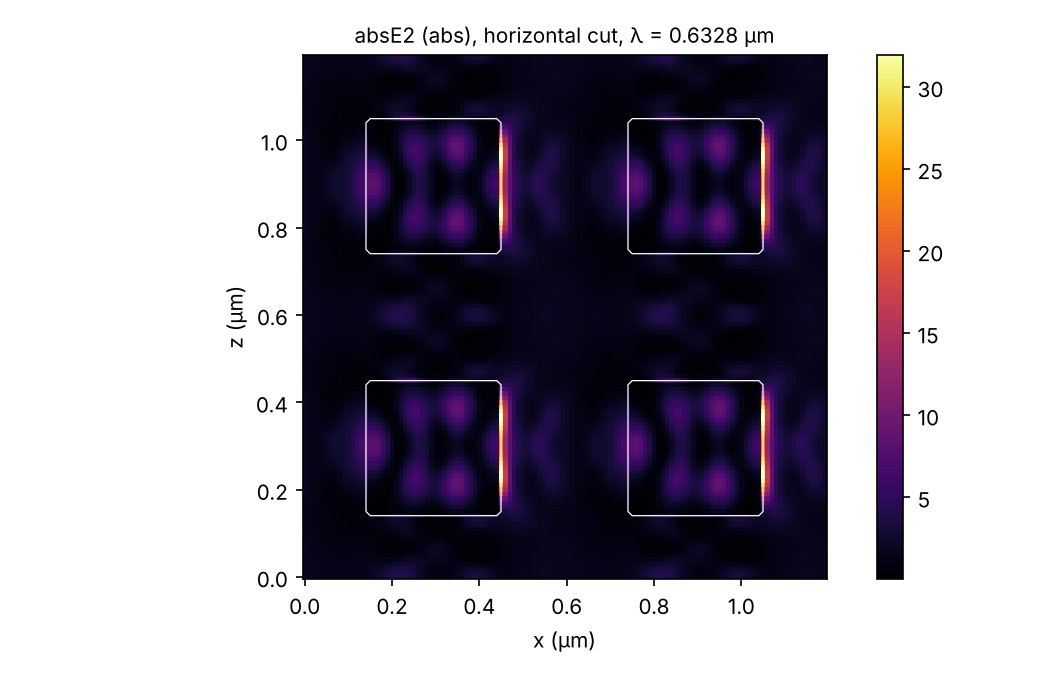
\includegraphics[width=0.6\linewidth]{fig/nf2d_horizontal.png}
\caption{Horizontaler Schnitt durch quadratische Siliziumsäulen (\file{examples/nearfield\_pillars\_2d.json}) in
halber Höhe, $|\mathbf E|^2$ über $x$ und $z$.}
\end{figure}

\section{Nahfeld in Python}
\begin{lstlisting}[style=py]
nf = fg.near_field(cfg)                      # Block "nearfield" der Konfiguration
v = nf["vertical"]
v["absE2"], v["Ex"], v["axis1_um"], v["axis2_um"], v["material"], v["meta"]
\end{lstlisting}
Die Arrays sind identisch mit den \file{.npy}-Dateien von \cmd{fgsolve}.

\section{Hinweise}
\begin{itemize}
  \item Die Auflösung \key{nx}, \key{ny} kostet kaum Rechenzeit; teuer ist die Rechnung selbst. Für Resonanzen
        lohnt sich ein höheres $N$ als für Effizienzen, weil lokale Feldspitzen langsamer konvergieren.
  \item Bei RCWA-Profilen ist das Feld innerhalb der Treppe die Lösung der Treppe, nicht des glatten Profils.
  \item Bei Metallen liegt das Feldmaximum oft an Kanten; dort konvergiert das Feld am langsamsten.
\end{itemize}
